\documentclass[11pt]{article}
%\usepackage[a3paper]{geometry}
%\usepackage[]{babel}
\usepackage[utf8]{inputenc}
\usepackage[T1]{fontenc}
\usepackage{fancyhdr}
\usepackage{graphicx}
\usepackage{amsmath}
\usepackage{amsfonts}
\usepackage{enumerate}
\usepackage{fancyvrb}
\usepackage[dvipsnames]{xcolor}
\PassOptionsToPackage{hyphens}{url}\usepackage{hyperref}
\usepackage {tikz}
\usetikzlibrary {positioning,fit,matrix,chains,calc,shapes.multipart,arrows,decorations.pathreplacing,shapes.arrows,chains,positioning}
\newlength\myht
\settoheight{\myht}{$n-2$}
%\usepackage{pgf}
%\usepgfplotslibrary{units}


\topmargin=0cm \oddsidemargin=0cm \evensidemargin=0cm \textheight=22cm
\textwidth=16cm \headheight=15pt \footskip=35pt

%\topmargin=0cm \oddsidemargin=0cm \evensidemargin=0cm \textheight=35cm
%\textwidth=25cm \headheight=15pt \footskip=35pt

\pagestyle{fancyplain}
\fancyhead{} % clear all header fields
\lhead{Enseirb-Matmeca M2 2021-2022}
\rhead{Quickly Différences Finies 2D}
\fancyfoot{} % clear all footer fields
\cfoot{\thepage}

\begin{document}

%headers
\begin{center}
{\bf \Large Quickly Différences Finies 2D } \\ 
N. Barral (\href{mailto:nicolas.barral@enseirb-matmeca.fr}{nicolas.barral@enseirb-matmeca.fr})
\end{center}
\hrule
\vspace*{1cm}

% beginning of the content

On considère un domaine rectangulaire $[x_{\min}, x_{\max}]\times[y_{\min}, y_{\max}]$ subdivisé en $N_x+1$ sous-intervalles de tailles égales selon les $x$ et $Ny+1$ sous-intervalles de tailles égales selon les $y$.

Dans la suite, on considerera le carré unité découpé comme sur la figure suivante:

\begin{figure}[!ht]
\center
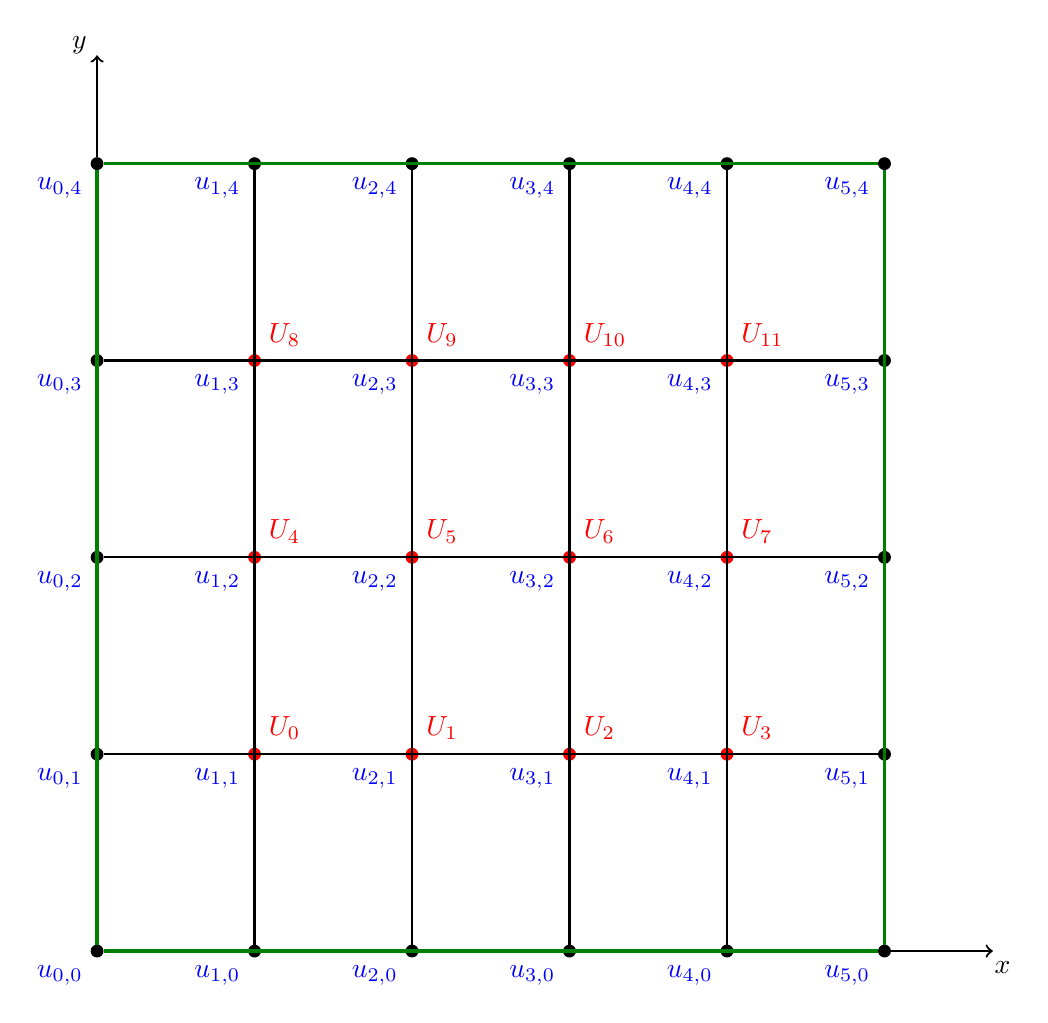
\begin{tikzpicture}[scale=1, , every node/.style={transform shape},
vertex/.style={circle, draw, fill, color=black, inner sep=1.5pt}]

\node[vertex, label={[blue]below left:$u_{0,0}$}] (1) at   (00.,00.0)     {};
\node[vertex, label={[blue]below left:$u_{0,1}$}] (2) at   (00.,02.5)     {};
\node[vertex, label={[blue]below left:$u_{0,2}$}] (3) at   (00.,05.0)     {};
\node[vertex, label={[blue]below left:$u_{0,3}$}] (4) at   (00.,07.5)     {};
\node[vertex, label={[blue]below left:$u_{0,4}$}] (5) at   (00.,10.0)     {};
\node[]       (5bis) at(00.,11.5)     {};
\node[vertex, label={[blue]below left:$u_{1,0}$}] (6) at   (02.,00.0)     {};
\node[vertex, red, label={[blue]below left:$u_{1,1}$}, label={[red]above right:$U_{0}$}] (7) at   (02.,02.5)     {};
\node[vertex, red, label={[blue]below left:$u_{1,2}$}, label={[red]above right:$U_{4}$}] (8) at   (02.,05.0)     {};
\node[vertex, red, label={[blue]below left:$u_{1,3}$}, label={[red]above right:$U_{8}$}] (9) at   (02.,07.5)     {};
\node[vertex, label={[blue]below left:$u_{1,4}$}] (10) at  (02.,10.0)     {};
\node[vertex, label={[blue]below left:$u_{2,0}$}] (11) at  (04.,00.0)     {};
\node[vertex, red, label={[blue]below left:$u_{2,1}$}, label={[red]above right:$U_{1}$}] (12) at  (04.,02.5)     {};
\node[vertex, red, label={[blue]below left:$u_{2,2}$}, label={[red]above right:$U_{5}$}] (13) at  (04.,05.0)     {};
\node[vertex, red, label={[blue]below left:$u_{2,3}$}, label={[red]above right:$U_{9}$}] (14) at  (04.,07.5)     {};
\node[vertex, label={[blue]below left:$u_{2,4}$}] (15) at  (04.,10.0)     {};
\node[vertex, label={[blue]below left:$u_{3,0}$}] (16) at  (06.,00.0)     {};
\node[vertex, red, label={[blue]below left:$u_{3,1}$}, label={[red]above right:$U_{2}$}] (17) at  (06.,02.5)     {};
\node[vertex, red, label={[blue]below left:$u_{3,2}$}, label={[red]above right:$U_{6}$}] (18) at  (06.,05.0)     {};
\node[vertex, red, label={[blue]below left:$u_{3,3}$}, label={[red]above right:$U_{10}$}] (19) at  (06.,07.5)     {};
\node[vertex, label={[blue]below left:$u_{3,4}$}] (20) at  (06.,10.0)     {};
\node[vertex, label={[blue]below left:$u_{4,0}$}] (21) at  (08.,00.0)     {};
\node[vertex, red, label={[blue]below left:$u_{4,1}$}, label={[red]above right:$U_{3}$}] (22) at  (08.,02.5)     {};
\node[vertex, red, label={[blue]below left:$u_{4,2}$}, label={[red]above right:$U_{7}$}] (23) at  (08.,05.0)     {};
\node[vertex, red, label={[blue]below left:$u_{4,3}$}, label={[red]above right:$U_{11}$}] (24) at  (08.,07.5)     {};
\node[vertex, label={[blue]below left:$u_{4,4}$}] (25) at  (08.,10.0)     {};
\node[vertex, label={[blue]below left:$u_{5,0}$}] (26) at  (10.,00.0)     {};
\node[]       (26bis) at(11.5,0.)     {};
\node[vertex, label={[blue]below left:$u_{5,1}$}] (27) at  (10.,02.5)     {};
\node[vertex, label={[blue]below left:$u_{5,2}$}] (28) at  (10.,05.0)     {};
\node[vertex, label={[blue]below left:$u_{5,3}$}] (29) at  (10.,07.5)     {};
\node[vertex, label={[blue]below left:$u_{5,4}$}] (30) at  (10.,10.0)     {};

\draw[very thick, black!50!green] (1) -- (5);
\draw[thick, ->] (5) -- (5bis) node[left]{$y$};
\draw[thick] (6) -- (10);
\draw[thick] (11) -- (15);
\draw[thick] (16) -- (20);
\draw[thick] (21) -- (25);
\draw[very thick, black!50!green] (26) -- (30);
\draw[very thick, black!50!green] (1) -- (26);
\draw[thick, ->] (26) -- (26bis) node[below]{$x$};
\draw[thick] (2) -- (27);
\draw[thick] (3) -- (28);
\draw[thick] (4) -- (29);
\draw[very thick, black!50!green] (5) -- (30);

\end{tikzpicture}
\caption{Maillage 2D d'un carré unité avec $N_x = 4$ et $N_y = 3$. La solution discrète $u$ de l'EDO est imposée en chaque sommet du bord (vert). En rouge, les degrés de liberté (inconnues) du problème numérotés avec un indice unique.}
\label{fig:mesh}
\end{figure}

On a : 
\begin{equation}
\begin{array}{l}
  x = x_{\min} + i\Delta x \, \\
  y = y_{\min} + j\Delta y \,
\end{array}
\end{equation}

On a également:
\begin{equation}
   I = (j-1)*N_x + (i-1) \textrm{\quad et \quad}
\begin{array}{lcll}
   j &=& \left\lfloor \frac{I}{N_x}\right\rfloor + 1 &\textrm{\ (division entière)}\\
   i &=& I \mod {N_x} + 1  &\textrm{\ (reste de la division)}
\end{array}
\label{eq:transfoIndices}
\end{equation}

\bigskip

On considère l'équation de la chaleur: 
\begin{equation}
	\left\{
	\begin{array}{l}
		\partial_t u - \sigma \Delta u = f\\
		\textrm{+ conditions aux bords} \,,	
	\end{array}
	\right.
\label{eq:heat}
\end{equation}
qui se discrétise sous la forme suivante, dans le cas d'un schéma en temps d'Euler explicite et d'une discrétisation centrée d'ordre 1 en espace:
\begin{equation}
  \frac{u^{n+1}_{i,j}-u^{n}_{i,j}}{\Delta t} + \sigma \frac{2u^{n}_{i,j}-u^{n}_{i+1,j}-u^{n}_{i-1,j}}{\Delta x^2} + \frac{2u^{n}_{i,j} - u^{n}_{i,j+1} - u^{n}_{i,j-1}}{\Delta y^2} = f^{n}_{i,j} \,.
\label{eq:discrete}
\end{equation}
Ce qui peut se réécrire:
\begin{equation}
 (u^{n+1}_{i,j}-u^{n}_{i,j}) + \sigma\Delta t\left(\alpha u^{n}_{i,j} - \beta u^{n}_{i+1,j} +  \beta u^{n}_{i-1,j} + \gamma u^{n}_{i,j+1} +  \gamma u^{n}_{i,j-1}\right) = \Delta t f^{n}_{i,j} \,,
\label{eq:discrete2}
\end{equation}
avec $\alpha = \frac{2}{\Delta x^2} + \frac{2}{\Delta y^2}$, $\beta = -\frac{2}{\Delta x^2}$ et $\gamma = -\frac{2}{\Delta y^2}$ \,.

\bigskip


Si on considère le cas de la Figure~\ref{fig:mesh}, $u$ est connue sur les bords (les conditions aux bords sont une donnée du problème), on écrit donc l'équation pour chaque point interne:
\begin{equation}
\left\{
\begin{array}{l}
(u^{n+1}_{1,1}-u^{n}_{1,1}) + \sigma\Delta t\left(\alpha u^{n}_{1,1} + \beta u^{n}_{2,1} +  \beta {\color{Green}u^{n}_{0,1}} +  \gamma u^{n}_{1,2} +  \gamma {\color{Green}u^{n}_{1,0}}\right) = \Delta t f^{n}_{1,1} \\ 
(u^{n+1}_{2,1}-u^{n}_{2,1}) + \sigma\Delta t\left(\alpha u^{n}_{2,1} + \beta u^{n}_{3,1} +  \beta u^{n}_{1,1} +  \gamma u^{n}_{2,2} +  \gamma {\color{Green}u^{n}_{2,0}}\right) = \Delta t f^{n}_{2,1} \\ 
(u^{n+1}_{3,1}-u^{n}_{3,1}) + \sigma\Delta t\left(\alpha u^{n}_{3,1} + \beta u^{n}_{4,1} +  \beta u^{n}_{2,1} +  \gamma u^{n}_{3,2} +  \gamma {\color{Green}u^{n}_{3,0}}\right) = \Delta t f^{n}_{3,1} \\ 
(u^{n+1}_{4,1}-u^{n}_{4,1}) + \sigma\Delta t\left(\alpha u^{n}_{4,1} + \beta {\color{Green}u^{n}_{5,1}} +  \beta u^{n}_{3,1} +  \gamma u^{n}_{4,2} +  \gamma {\color{Green}u^{n}_{4,0}}\right) = \Delta t f^{n}_{4,1} \\ 
(u^{n+1}_{1,2}-u^{n}_{1,2}) + \sigma\Delta t\left(\alpha u^{n}_{1,2} + \beta u^{n}_{2,2} +  \beta {\color{Green}u^{n}_{0,2}} +  \gamma u^{n}_{1,3} +  \gamma u^{n}_{1,1}\right) = \Delta t f^{n}_{1,2} \\ 
(u^{n+1}_{2,2}-u^{n}_{2,2}) + \sigma\Delta t\left(\alpha u^{n}_{2,2} + \beta u^{n}_{3,2} +  \beta u^{n}_{1,2} +  \gamma u^{n}_{2,3} +  \gamma u^{n}_{2,1}\right) = \Delta t f^{n}_{2,2} \\ 
(u^{n+1}_{3,2}-u^{n}_{3,2}) + \sigma\Delta t\left(\alpha u^{n}_{3,2} + \beta u^{n}_{4,2} +  \beta u^{n}_{2,2} +  \gamma u^{n}_{3,3} +  \gamma u^{n}_{3,1}\right) = \Delta t f^{n}_{3,2} \\ 
(u^{n+1}_{4,2}-u^{n}_{4,2}) + \sigma\Delta t\left(\alpha u^{n}_{4,2} + \beta {\color{Green}u^{n}_{5,2}} +  \beta u^{n}_{3,2} +  \gamma u^{n}_{4,3} +  \gamma u^{n}_{4,1}\right) = \Delta t f^{n}_{4,2} \\ 
(u^{n+1}_{1,3}-u^{n}_{1,3}) + \sigma\Delta t\left(\alpha u^{n}_{1,3} + \beta u^{n}_{2,3} +  \beta {\color{Green}u^{n}_{0,3}} +  \gamma {\color{Green}u^{n}_{1,4}} +  \gamma u^{n}_{1,2}\right) = \Delta t f^{n}_{1,3} \\ 
(u^{n+1}_{2,3}-u^{n}_{2,3}) + \sigma\Delta t\left(\alpha u^{n}_{2,3} + \beta u^{n}_{3,3} +  \beta u^{n}_{1,3} +  \gamma {\color{Green}u^{n}_{2,4}} +  \gamma u^{n}_{2,2}\right) = \Delta t f^{n}_{2,3} \\ 
(u^{n+1}_{3,3}-u^{n}_{3,3}) + \sigma\Delta t\left(\alpha u^{n}_{3,3} + \beta u^{n}_{4,3} +  \beta u^{n}_{2,3} +  \gamma {\color{Green}u^{n}_{3,4}} +  \gamma u^{n}_{3,2}\right) = \Delta t f^{n}_{3,3} \\ 
(u^{n+1}_{4,3}-u^{n}_{4,3}) + \sigma\Delta t\left(\alpha u^{n}_{4,3} + \beta {\color{Green}u^{n}_{5,3}} +  \beta u^{n}_{3,3} +  \gamma {\color{Green}u^{n}_{4,4}} +  \gamma u^{n}_{4,2}\right) = \Delta t f^{n}_{4,3} \,. 
\end{array}
\right. 
\end{equation}


Dans ce système, on va remplacer les termes en vert, qui correspondent aux sommets sur les bords, par leur valeur. Si on considère des conditions de Dirichlet homogènes nulles sur tout le bord, cela devient:
\begin{equation}
\left\{
\begin{array}{l}
(u^{n+1}_{1,1}-u^{n}_{1,1}) + \sigma\Delta t\left(\alpha u^{n}_{1,1} + \beta u^{n}_{2,1} +  {\color{Green}0} +  \gamma u^{n}_{1,2} +  {\color{Green}0}\right) = \Delta t f^{n}_{1,1} \\ 
(u^{n+1}_{2,1}-u^{n}_{2,1}) + \sigma\Delta t\left(\alpha u^{n}_{2,1} + \beta u^{n}_{3,1} +  \beta u^{n}_{1,1} +  \gamma u^{n}_{2,2} +  {\color{Green}0}\right) = \Delta t f^{n}_{2,1} \\ 
(u^{n+1}_{3,1}-u^{n}_{3,1}) + \sigma\Delta t\left(\alpha u^{n}_{3,1} + \beta u^{n}_{4,1} +  \beta u^{n}_{2,1} +  \gamma u^{n}_{3,2} +  {\color{Green}0}\right) = \Delta t f^{n}_{3,1} \\ 
(u^{n+1}_{4,1}-u^{n}_{4,1}) + \sigma\Delta t\left(\alpha u^{n}_{4,1} +  {\color{Green}0} +  \beta u^{n}_{3,1} +  \gamma u^{n}_{4,2} +  {\color{Green}0}\right) = \Delta t f^{n}_{4,1} \\ 
(u^{n+1}_{1,2}-u^{n}_{1,2}) + \sigma\Delta t\left(\alpha u^{n}_{1,2} + \beta u^{n}_{2,2} +   {\color{Green}0} +  \gamma u^{n}_{1,3} +  \gamma u^{n}_{1,1}\right) = \Delta t f^{n}_{1,2} \\ 
(u^{n+1}_{2,2}-u^{n}_{2,2}) + \sigma\Delta t\left(\alpha u^{n}_{2,2} + \beta u^{n}_{3,2} +  \beta u^{n}_{1,2} +  \gamma u^{n}_{2,3} +  \gamma u^{n}_{2,1}\right) = \Delta t f^{n}_{2,2} \\ 
(u^{n+1}_{3,2}-u^{n}_{3,2}) + \sigma\Delta t\left(\alpha u^{n}_{3,2} + \beta u^{n}_{4,2} +  \beta u^{n}_{2,2} +  \gamma u^{n}_{3,3} +  \gamma u^{n}_{3,1}\right) = \Delta t f^{n}_{3,2} \\ 
(u^{n+1}_{4,2}-u^{n}_{4,2}) + \sigma\Delta t\left(\alpha u^{n}_{4,2} +  {\color{Green}0} +  \beta u^{n}_{3,2} +  \gamma u^{n}_{4,3} +  \gamma u^{n}_{4,1}\right) = \Delta t f^{n}_{4,2} \\ 
(u^{n+1}_{1,3}-u^{n}_{1,3}) + \sigma\Delta t\left(\alpha u^{n}_{1,3} + \beta u^{n}_{2,3} +  {\color{Green}0} +  {\color{Green}0} +  \gamma u^{n}_{1,2}\right) = \Delta t f^{n}_{1,3} \\ 
(u^{n+1}_{2,3}-u^{n}_{2,3}) + \sigma\Delta t\left(\alpha u^{n}_{2,3} + \beta u^{n}_{3,3} +  \beta u^{n}_{1,3} +  {\color{Green}0} +  \gamma u^{n}_{2,2}\right) = \Delta t f^{n}_{2,3} \\ 
(u^{n+1}_{3,3}-u^{n}_{3,3}) + \sigma\Delta t\left(\alpha u^{n}_{3,3} + \beta u^{n}_{4,3} +  \beta u^{n}_{2,3} +  {\color{Green}0} +  \gamma u^{n}_{3,2}\right) = \Delta t f^{n}_{3,3} \\ 
(u^{n+1}_{4,3}-u^{n}_{4,3}) + \sigma\Delta t\left(\alpha u^{n}_{4,3} +  {\color{Green}0} +  \beta u^{n}_{3,3} +  {\color{Green}0} +  \gamma u^{n}_{4,2}\right) = \Delta t f^{n}_{4,3} \,.
\end{array}
\right.
\label{eq:system2}
\end{equation}

Pour les autres conditions au bord, il faudrait remplacer les termes en vert par autre chose (\emph{cf} slides de cours).

Informatiquement, il est parfois difficile de se repérer dans la grande matrice en utilisant i et j, on peut donc utiliser le I défini dans \ref{eq:transfoIndices}. On peut alors réécrire l'équation \ref{eq:discrete2}:

\begin{equation}
 (u^{n+1}_{I}-u^{n}_{I}) + \sigma\Delta t\left(\alpha u^{n}_{I} - \beta u^{n}_{I+1} +  \beta u^{n}_{I-1} + \gamma u^{n}_{I+N_x} +  \gamma u^{n}_{I-N_x}\right) = \Delta t f^{n}_{I} \,,
\label{eq:discrete3}
\end{equation}

et le système~\ref{eq:system2} devient:

\begin{equation}
\left\{
\begin{array}{l}
(u^{n+1}_{0}-u^{n}_{0}) + \sigma\Delta t\left(\alpha u^{n}_{0} + \beta u^{n}_{1} +  {\color{green}0} +  \gamma u^{n}_{4} +  {\color{green}0}\right) = f^{n}_{0} \\ 
(u^{n+1}_{1}-u^{n}_{1}) + \sigma\Delta t\left(\alpha u^{n}_{1} + \beta u^{n}_{2} +  \beta u^{n}_{0} +  \gamma u^{n}_{5} +  {\color{green}0}\right) = f^{n}_{1} \\ 
(u^{n+1}_{2}-u^{n}_{2}) + \sigma\Delta t\left(\alpha u^{n}_{2} + \beta u^{n}_{3} +  \beta u^{n}_{1} +  \gamma u^{n}_{6} +  {\color{green}0}\right) = f^{n}_{2} \\ 
(u^{n+1}_{3}-u^{n}_{3}) + \sigma\Delta t\left(\alpha u^{n}_{3} + {\color{green}0} +  \beta u^{n}_{2} +  \gamma u^{n}_{7} +  {\color{green}0}\right) = f^{n}_{3} \\ 
(u^{n+1}_{4}-u^{n}_{4}) + \sigma\Delta t\left(\alpha u^{n}_{4} + \beta u^{n}_{5} +  {\color{green}0} +  \gamma u^{n}_{8} +  \gamma u^{n}_{0}\right) = f^{n}_{4} \\ 
(u^{n+1}_{5}-u^{n}_{5}) + \sigma\Delta t\left(\alpha u^{n}_{5} + \beta u^{n}_{6} +  \beta u^{n}_{4} +  \gamma u^{n}_{9} +  \gamma u^{n}_{1}\right) = f^{n}_{5} \\ 
(u^{n+1}_{6}-u^{n}_{6}) + \sigma\Delta t\left(\alpha u^{n}_{6} + \beta u^{n}_{7} +  \beta u^{n}_{5} +  \gamma u^{n}_{10} +  \gamma u^{n}_{2}\right) = f^{n}_{6} \\ 
(u^{n+1}_{7}-u^{n}_{7}) + \sigma\Delta t\left(\alpha u^{n}_{7} + {\color{green}0} +  \beta u^{n}_{6} +  \gamma u^{n}_{11} +  \gamma u^{n}_{3}\right) = f^{n}_{7} \\ 
(u^{n+1}_{8}-u^{n}_{8}) + \sigma\Delta t\left(\alpha u^{n}_{8} + \beta u^{n}_{9} +  {\color{green}0} +  {\color{green}0} +  \gamma u^{n}_{4}\right) = f^{n}_{8} \\ 
(u^{n+1}_{9}-u^{n}_{9}) + \sigma\Delta t\left(\alpha u^{n}_{9} + \beta u^{n}_{10} +  \beta u^{n}_{8} +  {\color{green}0} +  \gamma u^{n}_{5}\right) = f^{n}_{9} \\ 
(u^{n+1}_{10}-u^{n}_{10}) + \sigma\Delta t\left(\alpha u^{n}_{10} + \beta u^{n}_{11} +  \beta u^{n}_{9} +  {\color{green}0} +  \gamma u^{n}_{6}\right) = f^{n}_{10} \\ 
(u^{n+1}_{11}-u^{n}_{11}) + \sigma\Delta t\left(\alpha u^{n}_{11} + {\color{green}0} +  \beta u^{n}_{10} +  {\color{green}0} +  \gamma u^{n}_{7}\right) = f^{n}_{11}  \,.
\end{array}
\right.
\end{equation}



Le système peut se réécrire sous la forme (faites le produit matrice-vecteur explicitement pour vous en convaincre!) :

\setcounter{MaxMatrixCols}{12}
\begin{equation}
\left(
\begin{array}{c}
u^{n+1}_{0}\\
u^{n+1}_{1}\\
u^{n+1}_{2}\\
u^{n+1}_{3}\\
u^{n+1}_{4}\\
u^{n+1}_{5}\\
u^{n+1}_{6}\\
u^{n+1}_{7}\\
u^{n+1}_{8}\\
u^{n+1}_{9}\\
u^{n+1}_{10}\\
u^{n+1}_{11}\\
\end{array}
\right)
-
\left(
\begin{array}{c}
u^{n}_{0}\\
u^{n}_{1}\\
u^{n}_{2}\\
u^{n}_{3}\\
u^{n}_{4}\\
u^{n}_{5}\\
u^{n}_{6}\\
u^{n}_{7}\\
u^{n}_{8}\\
u^{n}_{9}\\
u^{n}_{10}\\
u^{n}_{11}\\
\end{array}
\right)
+ 
\sigma \Delta t 
\begin{pmatrix}
\alpha & \beta & 0 & 0 & \gamma & 0 & 0 & 0 & 0 & 0 & 0 & 0 \\
\beta & \alpha & \beta & 0 & 0 & \gamma & 0 & 0 & 0 & 0 & 0 & 0 \\
0 & \beta & \alpha & \beta & 0 & 0 & \gamma & 0 & 0 & 0 & 0 & 0 \\
0 & 0 & \beta & \alpha & 0 & 0 & 0 & \gamma & 0 & 0 & 0 & 0 \\
\gamma & 0 & 0 & 0 & \alpha & \beta & 0 & 0 & \gamma & 0 & 0 & 0 \\
0 & \gamma & 0 & 0 & \beta & \alpha & \beta & 0 & 0 & \gamma & 0 & 0 \\
0 & 0 & \gamma & 0 & 0 & \beta & \alpha & \beta & 0 & 0 & \gamma & 0 \\
0 & 0 & 0 & \gamma & 0 & 0 & \beta & \alpha & 0 & 0 & 0 & \gamma \\
0 & 0 & 0 & 0 & \gamma & 0 & 0 & 0 & \alpha & \beta & 0 & 0 \\
0 & 0 & 0 & 0 & 0 & \gamma & 0 & 0 & \beta & \alpha & \beta & 0 \\
0 & 0 & 0 & 0 & 0 & 0 & \gamma & 0 & 0 & \beta & \alpha & \beta \\
0 & 0 & 0 & 0 & 0 & 0 & 0 & \gamma & 0 & 0 & \beta & \alpha \\

\end{pmatrix}
\left(
\begin{array}{c}
u^{n}_{0}\\
u^{n}_{1}\\
u^{n}_{2}\\
u^{n}_{3}\\
u^{n}_{4}\\
u^{n}_{5}\\
u^{n}_{6}\\
u^{n}_{7}\\
u^{n}_{8}\\
u^{n}_{9}\\
u^{n}_{10}\\
u^{n}_{11}\\
\end{array}
\right)
=
\Delta t 
\left(
\begin{array}{c}
f^{n}_{0}\\
f^{n}_{1}\\
f^{n}_{2}\\
f^{n}_{3}\\
f^{n}_{4}\\
f^{n}_{5}\\
f^{n}_{6}\\
f^{n}_{7}\\
f^{n}_{8}\\
f^{n}_{9}\\
f^{n}_{10}\\
f^{n}_{11}\\
\end{array}
\right) \,,
\label{eq:sysMat2}
\end{equation}
%\begin{equation}
%\left(
%\begin{array}{c}
%u^{n+1}_{1,1}\\
%u^{n+1}_{2,1}\\
%u^{n+1}_{3,1}\\
%u^{n+1}_{4,1}\\
%u^{n+1}_{1,2}\\
%u^{n+1}_{2,2}\\
%u^{n+1}_{3,2}\\
%u^{n+1}_{4,2}\\
%u^{n+1}_{1,3}\\
%u^{n+1}_{2,3}\\
%u^{n+1}_{3,3}\\
%u^{n+1}_{4,3}\\
%\end{array}
%\right)
%-
%\left(
%\begin{array}{c}
%u^{n}_{1,1}\\
%u^{n}_{2,1}\\
%u^{n}_{3,1}\\
%u^{n}_{4,1}\\
%u^{n}_{1,2}\\
%u^{n}_{2,2}\\
%u^{n}_{3,2}\\
%u^{n}_{4,2}\\
%u^{n}_{1,3}\\
%u^{n}_{2,3}\\
%u^{n}_{3,3}\\
%u^{n}_{4,3}\\
%\end{array}
%\right)
%+ 
%\sigma \Delta t 
%\begin{pmatrix}
%\alpha & \beta & 0 & 0 & \gamma & 0 & 0 & 0 & 0 & 0 & 0 & 0 \\
%\beta & \alpha & \beta & 0 & 0 & \gamma & 0 & 0 & 0 & 0 & 0 & 0 \\
%0 & \beta & \alpha & \beta & 0 & 0 & \gamma & 0 & 0 & 0 & 0 & 0 \\
%0 & 0 & \beta & \alpha & 0 & 0 & 0 & \gamma & 0 & 0 & 0 & 0 \\
%\gamma & 0 & 0 & 0 & \alpha & \beta & 0 & 0 & \gamma & 0 & 0 & 0 \\
%0 & \gamma & 0 & 0 & \beta & \alpha & \beta & 0 & 0 & \gamma & 0 & 0 \\
%0 & 0 & \gamma & 0 & 0 & \beta & \alpha & \beta & 0 & 0 & \gamma & 0 \\
%0 & 0 & 0 & \gamma & 0 & 0 & \beta & \alpha & 0 & 0 & 0 & \gamma \\
%0 & 0 & 0 & 0 & \gamma & 0 & 0 & 0 & \alpha & \beta & 0 & 0 \\
%0 & 0 & 0 & 0 & 0 & \gamma & 0 & 0 & \beta & \alpha & \beta & 0 \\
%0 & 0 & 0 & 0 & 0 & 0 & \gamma & 0 & 0 & \beta & \alpha & \beta \\
%0 & 0 & 0 & 0 & 0 & 0 & 0 & \gamma & 0 & 0 & \beta & \alpha \\
%
%\end{pmatrix}
%\left(
%\begin{array}{c}
%u^{n}_{1,1}\\
%u^{n}_{2,1}\\
%u^{n}_{3,1}\\
%u^{n}_{4,1}\\
%u^{n}_{1,2}\\
%u^{n}_{2,2}\\
%u^{n}_{3,2}\\
%u^{n}_{4,2}\\
%u^{n}_{1,3}\\
%u^{n}_{2,3}\\
%u^{n}_{3,3}\\
%u^{n}_{4,3}\\
%\end{array}
%\right)
%=
%\Delta t 
%\left(
%\begin{array}{c}
%f^{n}_{1,1}\\
%f^{n}_{2,1}\\
%f^{n}_{3,1}\\
%f^{n}_{4,1}\\
%f^{n}_{1,2}\\
%f^{n}_{2,2}\\
%f^{n}_{3,2}\\
%f^{n}_{4,2}\\
%f^{n}_{1,3}\\
%f^{n}_{2,3}\\
%f^{n}_{3,3}\\
%f^{n}_{4,3}\\
%\end{array}
%\right)
%\label{eq:sysMat1}
%\end{equation}

soit

\begin{equation}
U^{n+1} - U^{n} + \sigma\Delta t \mathbb{H} U^{n} = \Delta t F^{n} \,.
\end{equation}

Chaque ligne de la matrice correspond à donc l'équation \ref{eq:discrete2} écrite pour un sommet du maillage donné : La ligne I de la matrice correspond donc à l'équation~\ref{eq:discrete3} écrite pour le I-ème degré de liberté du système. L'élément (I, J) de la matrice correspond à la contribution de $U_J$ à la ligne pour $U_I$. Si le sommet est près d'un bord, certains termes de l'équation doivent être remplacés par des conditions aux bords, ce qui change la ligne correspondante pour la matrice et le second membre.


\bigskip


En pratique, pour former la matrice et le second membre, on a donc le choix entre deux façons de boucler:

\fvset{frame=single, label=Première construction de la boucle}
\begin{Verbatim}
vector<Triplet<double>> triplets;
for (int I=0; I<Nx*Ny; ++I) {
    i = I%Nx + 1; // modulo
    j = I/Nx + 1; // division entière
    triplets.push_back({I, I, ...});
    if (i > 1) {  // Le sommet n'est pas près d'un bord gauche
        triplets.push_back({I, I-1, ...});
    }
    if (i < Nx) {  // Le sommet n'est pas près d'un bord droit
        triplets.push_back({I, I+1, ...});
    } 
    ...
}
_H.setFromTriplets(triplets.begin(), triplets.end());
\end{Verbatim}

ou

\fvset{frame=single, label=Deuxième construction de la boucle}
\begin{Verbatim}
vector<Triplet<double>> triplets;
for (int j=1; j<=Ny; ++j) {
    for (int i=1; i<=Nx; ++i) {
        I = (j-1)*Nx + i-1
        triplets.push_back({I, I, ...});
        if (i > 1) {  // Le sommet n'est pas près d'un bord gauche
            triplets.push_back({I, I-1, ...});
        }
        if (i < Nx) {  // Le sommet n'est pas près d'un bord droit
            triplets.push_back({I, I+1, ...});
        } 
        ...
    }
}
_H.setFromTriplets(triplets.begin(), triplets.end());
\end{Verbatim}

Ces deux façons sont équivalentes, c'est à vous de voir celle avec laquelle vous êtes la plus à l'aise.

Pour la formation du second membre, c'est la même chose: on boucle sur les inconnues, et en fonction de leur place sur la grille et du type de condition aux bords, on rajoute des termes.

\end{document}
